\documentclass[11pt]{article}
\usepackage[a4paper,margin=0.75in]{geometry}
\usepackage{amsmath}
\usepackage{epsfig}
\usepackage{subcaption}
\usepackage[section]{placeins}
\usepackage{framed}
\usepackage{hyperref}
\nocite{*}
\newtheorem{theorem}{Theorem}[section]
\begin{document}
\title{All about triangles}
\author{Apoorv Khurasia}
\maketitle
\section{What is a triangle?}
A triangle is a polygon with three straight sides.
\begin{figure}[!htb]
    \centering
    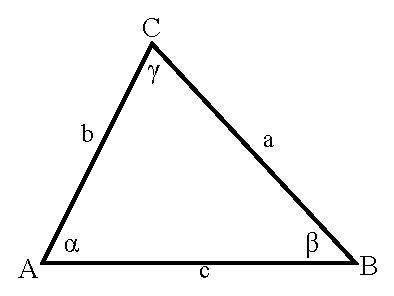
\includegraphics{triangle_basics.eps}
    \caption{A triangle}
    \label{fig:triangle}
\end{figure}
Let's get used to some notation. In Fig. \ref{fig:triangle}, the vertices of the triangle are denoted by $A$, $B$, and $C$. It is customary to use uppercase Latin alphabet to label vertices of polygons. The sides opposite to these vertices are denoted by $a$, $b$, and $c$ respectively. The angles at these vertices are denoted by $\alpha$, $\beta$, and $\gamma$. It is customary to use lowercase Greek alphabet to denote angles in polygons. The triangle itself is denoted by $\triangle ABC$.
\newline
We also use the following notation:
\begin{itemize}
    \item $AB$ denotes the line segment joining points $A$ and $B$ and $\overline{AB}$ denotes the length of that segment. Obviously, $\overline{AB} = c$. Similarly, $\overline{BC} = a$ and $\overline{CA} = b$.
    \item $\angle ABC$ denotes the angle at vertex $B$ formed by line segments $AB$ and $BC$ and is equal to $\beta$. Similarly, $\angle BCA = \gamma$ and $\angle CAB = \alpha$.
    \item The perimeter of a triangle is the sum of the lengths of all its sides. For our $\triangle ABC$, it is $a + b + c$. The semi-perimeter (or half-perimeter) of $\triangle ABC$ is denoted by:
          \begin{equation*}s = \frac{a + b + c}{2}\end{equation*}
\end{itemize}
An important property of triangles is that the sum of the angles in a triangle is always $180^\circ$. This is a provable statement and in mathematics, we call such statements \textbf{theorems} and state them like so:
\begin{theorem}
    The sum of the (interior) angles in a triangle is $180^\circ$.
    \label{thm:triangle_angles}
\end{theorem}
We have specified that the angles are interior angles. This is because a triangle can also have exterior angles, which are formed by extending one of its sides. The sum of the exterior angles of a triangle is always $360^\circ$.
\begin{framed}
    \textbf{Exercise:} First, draw a triangle and measure its angles. Verify this theorem. But all you would have done is verify this theorem for a single triangle. Can you prove that this theorem holds for all triangles? \textit{Hint: Use the fact that the sum of angles on a straight line is $180^\circ$}.
\end{framed}
\newpage
\section{Types of triangles}
Triangles can be classified based on their angles and sides.
\subsection{Based on angles}
Triangles can be classified based on their angles:
\begin{figure*}[!htbp]
    \centering
    \begin{subfigure}[t]{0.3\textwidth}
        \centering
        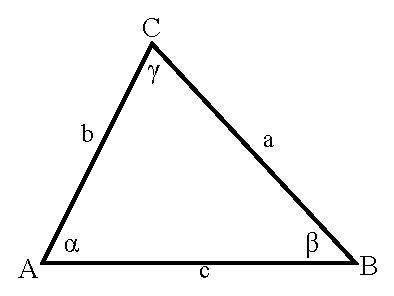
\includegraphics[scale=0.7]{triangle_basics.eps}
        \caption{An \textbf{acute triangle} has all angles less than $90^\circ$.}
    \end{subfigure}
    ~
    \begin{subfigure}[t]{0.3\textwidth}
        \centering
        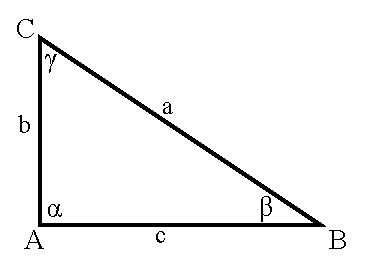
\includegraphics[scale=0.7]{right_triangle.eps}
        \caption{A \textbf{right triangle} has one angle equal to $90^\circ$. Here, $\angle BAC = \alpha = 90^\circ$.}
        \label{fig:right_triangle}
    \end{subfigure}%
    ~
    \begin{subfigure}[t]{0.3\textwidth}
        \centering
        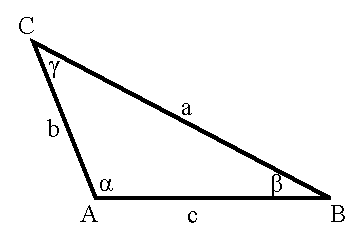
\includegraphics[scale=0.7]{obtuse_triangle.eps}
        \caption{An \textbf{obtuse triangle} has one angle greater than $90^\circ$. Here, $\angle BAC = \alpha > 90^\circ$.}
        \label{fig:obtuse_triangle}
    \end{subfigure}
    \caption{Different types of triangles based on angles}
\end{figure*}
\FloatBarrier
\subsection{Based on sides}
Triangles can also be classified based on the lengths of their sides. The hatches in the figure below denote the sides that are equal to one another.
\begin{figure*}[!htbp]
    \centering
    \begin{subfigure}[t]{0.49\textwidth}
        \centering
        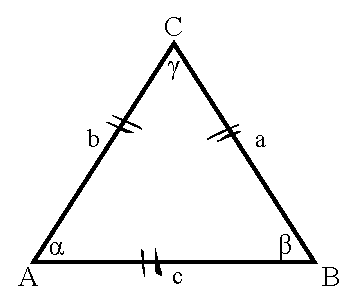
\includegraphics[scale=0.7]{equilateral_triangle.eps}
        \caption{An \textbf{equilateral triangle} has all its sides equal. Here, $\overline{AB} = \overline{BC} = \overline{CA}$.}
        \label{fig:equilateral_triangle}
    \end{subfigure}
    ~
    \begin{subfigure}[t]{0.49\textwidth}
        \centering
        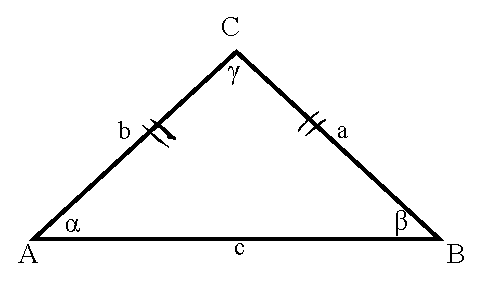
\includegraphics[scale=0.7]{isosceles.eps}
        \caption{An \textbf{isosceles triangle} has two angles equal. Here, $\overline{AC} = \overline{BC} \neq \overline{AB}$.}
        \label{fig:isosceles_triangle}
    \end{subfigure}%
    \caption{Different types of triangles based on sides}
\end{figure*}
\FloatBarrier
\subsection{Exercises}
Using Theorem \ref{thm:triangle_angles}, let's try to answer the following questions:
\begin{framed}
    \begin{enumerate}
        \item Can a triangle have two right angles? Why or why not?
        \item Can a triangle have two obtuse angles? Why or why not?
        \item Can a triangle have two acute angles? Why or why not?
    \end{enumerate}
\end{framed}
\newpage
\section{More properties of triangles}
Here are some relationships between the sides and angles of triangles that are useful to know.
\begin{enumerate}
    \item The sum of the lengths of any two sides of a triangle is greater than the length of the third side. This is known as the \textbf{triangle inequality property}. Therefore, in any $\triangle ABC$:
          \begin{equation*}
              \overline{AB} + \overline{BC} > \overline{AC}, \quad \overline{AC} + \overline{BC} > \overline{AB}, \quad \overline{AB} + \overline{AC} > \overline{BC}
          \end{equation*}
    \item \begin{theorem} Angles opposite to equal sides of a triangle are equal. This is known as the \textbf{isosceles triangle theorem}. In any $\triangle ABC$,
              \begin{equation*}
                  \text{If } \overline{AB} = \overline{AC}, \text{ then } \angle ABC = \angle ACB
              \end{equation*}
              \label{thm:isosceles_triangle}
          \end{theorem}
          When mathematicians write a statement using \textit{if} like here, they mean that "whenever the condition on the left-hand side is true, the conclusion on the right-hand side is also true". In this case, it means that whenever $\overline{AB} = \overline{AC}$, then $\angle ABC$ must equal $\angle ACB$.
    \item \begin{theorem} Angles opposite to a larger side of a triangle are larger than those opposite to a smaller side. In any $\triangle ABC$,
              \begin{equation*}
                  \text{If } \overline{AB} > \overline{AC}, \text{ then } \angle ACB > \angle ABC
              \end{equation*}
              \label{thm:larger_side_larger_angle_triangle}
          \end{theorem}
\end{enumerate}
\subsection{Exercises}
\begin{framed}
    \begin{enumerate}
        \item Can you prove theorems \ref{thm:isosceles_triangle} and \ref{thm:larger_side_larger_angle_triangle} in this list above?
        \item Prove that the angles opposite to equal sides of a triangle are equal using the isosceles triangle theorem.
        \item Prove that all angles of an equilateral triangle are equal.
        \item In Fig. \ref{fig:isosceles_triangle}, $AB$ is the largest side. Which is the largest angle?
        \item Can a triangle with sides 4 cm, 5 cm, and 6 cm exist? Why or why not?
        \item Can a triangle with sides 2 cm, 3 cm, and 6 cm exist? Why or why not?
    \end{enumerate}
\end{framed}
\end{document}